\section*{RESULTS}
Empty section :)

The problem described above was solved using Hermes2D.  The solution $\phi(x,y)$ at time level $t=0.1 \mbox{ s}$ is shown in figure \ref{sol_temp}.

\begin{figure}
  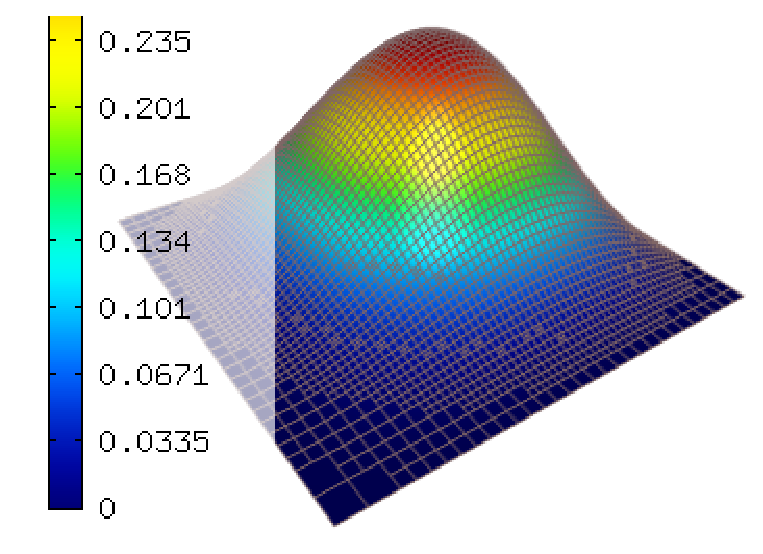
\includegraphics[width=0.5\textwidth]{figures/solution_T}
  \caption{h-mesh (linear elements, p=2) for the neutron flux at time level $t=0.1 \mbox{ s}$.  Solution for $\phi$ contains 60353 DOFs and has a relative error 0.00019 \%.}
  \label{sol_temp}
\end{figure}

using both hp-adaptation and uniform refinement with linear and quadratic finite elements.

compare the numerical results with the analytical solution

The relative error in $L_2$ norm, between the numerical results $v$ and the analytical solution $v_{exact}$ is computed using
\begin{align}
  e = \frac{ \|v-v_{exact}\|_{L_2} }{ \|v_{exact}\|_{L_2} }
\end{align}

Figure \ref{err_conv} shows the error for the temperature $T^{n}(x,y)$ at fixed time level $n$.


The manufactured solition is a continuum solution, and thus can be evaluated at the same time and space points as the computed solution.

convergence study

shows the approximation error in logarithmic scale
\begin{figure}
  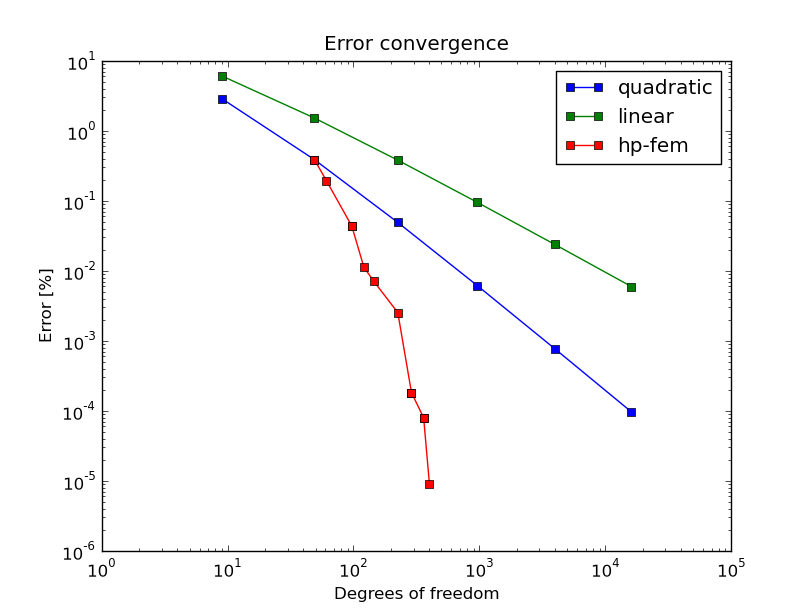
\includegraphics[width=0.5\textwidth]{figures/exact_err_conv}
  \caption{Convergence comparison of adaptive hp-FEM with linar and quadratic finite elements.  (exact error in norm $L_2$ for the temperature $T$)}
  \label{err_conv}
\end{figure}
since exact solution is available, compute both estimated error (via the reference solution) as well as the exact error.  Thus one can see the quality of the error estimate.  Note that the estimated error usually is slightly less than the exact one, but during adaptivity they quickly converge together and become virtually identical. This is shown in the figure below.

Comparison of h-FEM with linear and quadratic elements, and the hp-FEM on a log-log scale.

Same graphs as above but now in terms of CPU time

